% Generated by Sphinx.
\def\sphinxdocclass{report}
\documentclass[a4paper,12pt,spanish]{sphinxmanual}
\usepackage[utf8]{inputenc}
\DeclareUnicodeCharacter{00A0}{\nobreakspace}
\usepackage{cmap}
\usepackage[T1]{fontenc}
\usepackage{babel}
\usepackage{times}
\usepackage[Sonny]{fncychap}
\usepackage{longtable}
\usepackage{sphinx}
\usepackage{multirow}

  \setcounter{tocdepth}{2}
  \fancypagestyle{normal}{
    \fancyhf{}
    % Footer

    \fancyfoot[LE,RO]{{\textbf{\textsf{\thepage}}}}
    \fancyfoot[LO]{{\sffamily\bfseries\nouppercase{\textbf{\rightmark}}}}
    \fancyfoot[RE]{{\sffamily\bfseries\nouppercase{\textbf{\leftmark}}}}

    \fancyhead[LE,RO]{{\sffamily\bfseries\nouppercase{\textit{Introducción al desarrollo de software}}}}

    \renewcommand{\headrulewidth}{0.4pt}
    \renewcommand{\footrulewidth}{0.4pt}
  }
  % Update the plain style so we get the page number & footer line,
  % but not a chapter or section title.  This is to keep the first
  % page of a chapter and the blank page between chapters `clean.'
  \fancypagestyle{plain}{
    \fancyhf{}
    \fancyfoot[RO,RE]{{\textbf{\textsf{\thepage}}}}
    \renewcommand{\headrulewidth}{0pt}
    \renewcommand{\footrulewidth}{0.4pt}
  }


\title{Introducción al desarrollo de software}
\date{19 de May de 2015}
\release{1.0}
\author{Emiliano López}
\newcommand{\sphinxlogo}{}
\renewcommand{\releasename}{Publicación}
\makeindex

\makeatletter
\def\PYG@reset{\let\PYG@it=\relax \let\PYG@bf=\relax%
    \let\PYG@ul=\relax \let\PYG@tc=\relax%
    \let\PYG@bc=\relax \let\PYG@ff=\relax}
\def\PYG@tok#1{\csname PYG@tok@#1\endcsname}
\def\PYG@toks#1+{\ifx\relax#1\empty\else%
    \PYG@tok{#1}\expandafter\PYG@toks\fi}
\def\PYG@do#1{\PYG@bc{\PYG@tc{\PYG@ul{%
    \PYG@it{\PYG@bf{\PYG@ff{#1}}}}}}}
\def\PYG#1#2{\PYG@reset\PYG@toks#1+\relax+\PYG@do{#2}}

\expandafter\def\csname PYG@tok@gd\endcsname{\def\PYG@tc##1{\textcolor[rgb]{0.63,0.00,0.00}{##1}}}
\expandafter\def\csname PYG@tok@gu\endcsname{\let\PYG@bf=\textbf\def\PYG@tc##1{\textcolor[rgb]{0.50,0.00,0.50}{##1}}}
\expandafter\def\csname PYG@tok@gt\endcsname{\def\PYG@tc##1{\textcolor[rgb]{0.00,0.27,0.87}{##1}}}
\expandafter\def\csname PYG@tok@gs\endcsname{\let\PYG@bf=\textbf}
\expandafter\def\csname PYG@tok@gr\endcsname{\def\PYG@tc##1{\textcolor[rgb]{1.00,0.00,0.00}{##1}}}
\expandafter\def\csname PYG@tok@cm\endcsname{\let\PYG@it=\textit\def\PYG@tc##1{\textcolor[rgb]{0.25,0.50,0.56}{##1}}}
\expandafter\def\csname PYG@tok@vg\endcsname{\def\PYG@tc##1{\textcolor[rgb]{0.73,0.38,0.84}{##1}}}
\expandafter\def\csname PYG@tok@m\endcsname{\def\PYG@tc##1{\textcolor[rgb]{0.13,0.50,0.31}{##1}}}
\expandafter\def\csname PYG@tok@mh\endcsname{\def\PYG@tc##1{\textcolor[rgb]{0.13,0.50,0.31}{##1}}}
\expandafter\def\csname PYG@tok@cs\endcsname{\def\PYG@tc##1{\textcolor[rgb]{0.25,0.50,0.56}{##1}}\def\PYG@bc##1{\setlength{\fboxsep}{0pt}\colorbox[rgb]{1.00,0.94,0.94}{\strut ##1}}}
\expandafter\def\csname PYG@tok@ge\endcsname{\let\PYG@it=\textit}
\expandafter\def\csname PYG@tok@vc\endcsname{\def\PYG@tc##1{\textcolor[rgb]{0.73,0.38,0.84}{##1}}}
\expandafter\def\csname PYG@tok@il\endcsname{\def\PYG@tc##1{\textcolor[rgb]{0.13,0.50,0.31}{##1}}}
\expandafter\def\csname PYG@tok@go\endcsname{\def\PYG@tc##1{\textcolor[rgb]{0.20,0.20,0.20}{##1}}}
\expandafter\def\csname PYG@tok@cp\endcsname{\def\PYG@tc##1{\textcolor[rgb]{0.00,0.44,0.13}{##1}}}
\expandafter\def\csname PYG@tok@gi\endcsname{\def\PYG@tc##1{\textcolor[rgb]{0.00,0.63,0.00}{##1}}}
\expandafter\def\csname PYG@tok@gh\endcsname{\let\PYG@bf=\textbf\def\PYG@tc##1{\textcolor[rgb]{0.00,0.00,0.50}{##1}}}
\expandafter\def\csname PYG@tok@ni\endcsname{\let\PYG@bf=\textbf\def\PYG@tc##1{\textcolor[rgb]{0.84,0.33,0.22}{##1}}}
\expandafter\def\csname PYG@tok@nl\endcsname{\let\PYG@bf=\textbf\def\PYG@tc##1{\textcolor[rgb]{0.00,0.13,0.44}{##1}}}
\expandafter\def\csname PYG@tok@nn\endcsname{\let\PYG@bf=\textbf\def\PYG@tc##1{\textcolor[rgb]{0.05,0.52,0.71}{##1}}}
\expandafter\def\csname PYG@tok@no\endcsname{\def\PYG@tc##1{\textcolor[rgb]{0.38,0.68,0.84}{##1}}}
\expandafter\def\csname PYG@tok@na\endcsname{\def\PYG@tc##1{\textcolor[rgb]{0.25,0.44,0.63}{##1}}}
\expandafter\def\csname PYG@tok@nb\endcsname{\def\PYG@tc##1{\textcolor[rgb]{0.00,0.44,0.13}{##1}}}
\expandafter\def\csname PYG@tok@nc\endcsname{\let\PYG@bf=\textbf\def\PYG@tc##1{\textcolor[rgb]{0.05,0.52,0.71}{##1}}}
\expandafter\def\csname PYG@tok@nd\endcsname{\let\PYG@bf=\textbf\def\PYG@tc##1{\textcolor[rgb]{0.33,0.33,0.33}{##1}}}
\expandafter\def\csname PYG@tok@ne\endcsname{\def\PYG@tc##1{\textcolor[rgb]{0.00,0.44,0.13}{##1}}}
\expandafter\def\csname PYG@tok@nf\endcsname{\def\PYG@tc##1{\textcolor[rgb]{0.02,0.16,0.49}{##1}}}
\expandafter\def\csname PYG@tok@si\endcsname{\let\PYG@it=\textit\def\PYG@tc##1{\textcolor[rgb]{0.44,0.63,0.82}{##1}}}
\expandafter\def\csname PYG@tok@s2\endcsname{\def\PYG@tc##1{\textcolor[rgb]{0.25,0.44,0.63}{##1}}}
\expandafter\def\csname PYG@tok@vi\endcsname{\def\PYG@tc##1{\textcolor[rgb]{0.73,0.38,0.84}{##1}}}
\expandafter\def\csname PYG@tok@nt\endcsname{\let\PYG@bf=\textbf\def\PYG@tc##1{\textcolor[rgb]{0.02,0.16,0.45}{##1}}}
\expandafter\def\csname PYG@tok@nv\endcsname{\def\PYG@tc##1{\textcolor[rgb]{0.73,0.38,0.84}{##1}}}
\expandafter\def\csname PYG@tok@s1\endcsname{\def\PYG@tc##1{\textcolor[rgb]{0.25,0.44,0.63}{##1}}}
\expandafter\def\csname PYG@tok@gp\endcsname{\let\PYG@bf=\textbf\def\PYG@tc##1{\textcolor[rgb]{0.78,0.36,0.04}{##1}}}
\expandafter\def\csname PYG@tok@sh\endcsname{\def\PYG@tc##1{\textcolor[rgb]{0.25,0.44,0.63}{##1}}}
\expandafter\def\csname PYG@tok@ow\endcsname{\let\PYG@bf=\textbf\def\PYG@tc##1{\textcolor[rgb]{0.00,0.44,0.13}{##1}}}
\expandafter\def\csname PYG@tok@sx\endcsname{\def\PYG@tc##1{\textcolor[rgb]{0.78,0.36,0.04}{##1}}}
\expandafter\def\csname PYG@tok@bp\endcsname{\def\PYG@tc##1{\textcolor[rgb]{0.00,0.44,0.13}{##1}}}
\expandafter\def\csname PYG@tok@c1\endcsname{\let\PYG@it=\textit\def\PYG@tc##1{\textcolor[rgb]{0.25,0.50,0.56}{##1}}}
\expandafter\def\csname PYG@tok@kc\endcsname{\let\PYG@bf=\textbf\def\PYG@tc##1{\textcolor[rgb]{0.00,0.44,0.13}{##1}}}
\expandafter\def\csname PYG@tok@c\endcsname{\let\PYG@it=\textit\def\PYG@tc##1{\textcolor[rgb]{0.25,0.50,0.56}{##1}}}
\expandafter\def\csname PYG@tok@mf\endcsname{\def\PYG@tc##1{\textcolor[rgb]{0.13,0.50,0.31}{##1}}}
\expandafter\def\csname PYG@tok@err\endcsname{\def\PYG@bc##1{\setlength{\fboxsep}{0pt}\fcolorbox[rgb]{1.00,0.00,0.00}{1,1,1}{\strut ##1}}}
\expandafter\def\csname PYG@tok@mb\endcsname{\def\PYG@tc##1{\textcolor[rgb]{0.13,0.50,0.31}{##1}}}
\expandafter\def\csname PYG@tok@ss\endcsname{\def\PYG@tc##1{\textcolor[rgb]{0.32,0.47,0.09}{##1}}}
\expandafter\def\csname PYG@tok@sr\endcsname{\def\PYG@tc##1{\textcolor[rgb]{0.14,0.33,0.53}{##1}}}
\expandafter\def\csname PYG@tok@mo\endcsname{\def\PYG@tc##1{\textcolor[rgb]{0.13,0.50,0.31}{##1}}}
\expandafter\def\csname PYG@tok@kd\endcsname{\let\PYG@bf=\textbf\def\PYG@tc##1{\textcolor[rgb]{0.00,0.44,0.13}{##1}}}
\expandafter\def\csname PYG@tok@mi\endcsname{\def\PYG@tc##1{\textcolor[rgb]{0.13,0.50,0.31}{##1}}}
\expandafter\def\csname PYG@tok@kn\endcsname{\let\PYG@bf=\textbf\def\PYG@tc##1{\textcolor[rgb]{0.00,0.44,0.13}{##1}}}
\expandafter\def\csname PYG@tok@o\endcsname{\def\PYG@tc##1{\textcolor[rgb]{0.40,0.40,0.40}{##1}}}
\expandafter\def\csname PYG@tok@kr\endcsname{\let\PYG@bf=\textbf\def\PYG@tc##1{\textcolor[rgb]{0.00,0.44,0.13}{##1}}}
\expandafter\def\csname PYG@tok@s\endcsname{\def\PYG@tc##1{\textcolor[rgb]{0.25,0.44,0.63}{##1}}}
\expandafter\def\csname PYG@tok@kp\endcsname{\def\PYG@tc##1{\textcolor[rgb]{0.00,0.44,0.13}{##1}}}
\expandafter\def\csname PYG@tok@w\endcsname{\def\PYG@tc##1{\textcolor[rgb]{0.73,0.73,0.73}{##1}}}
\expandafter\def\csname PYG@tok@kt\endcsname{\def\PYG@tc##1{\textcolor[rgb]{0.56,0.13,0.00}{##1}}}
\expandafter\def\csname PYG@tok@sc\endcsname{\def\PYG@tc##1{\textcolor[rgb]{0.25,0.44,0.63}{##1}}}
\expandafter\def\csname PYG@tok@sb\endcsname{\def\PYG@tc##1{\textcolor[rgb]{0.25,0.44,0.63}{##1}}}
\expandafter\def\csname PYG@tok@k\endcsname{\let\PYG@bf=\textbf\def\PYG@tc##1{\textcolor[rgb]{0.00,0.44,0.13}{##1}}}
\expandafter\def\csname PYG@tok@se\endcsname{\let\PYG@bf=\textbf\def\PYG@tc##1{\textcolor[rgb]{0.25,0.44,0.63}{##1}}}
\expandafter\def\csname PYG@tok@sd\endcsname{\let\PYG@it=\textit\def\PYG@tc##1{\textcolor[rgb]{0.25,0.44,0.63}{##1}}}

\def\PYGZbs{\char`\\}
\def\PYGZus{\char`\_}
\def\PYGZob{\char`\{}
\def\PYGZcb{\char`\}}
\def\PYGZca{\char`\^}
\def\PYGZam{\char`\&}
\def\PYGZlt{\char`\<}
\def\PYGZgt{\char`\>}
\def\PYGZsh{\char`\#}
\def\PYGZpc{\char`\%}
\def\PYGZdl{\char`\$}
\def\PYGZhy{\char`\-}
\def\PYGZsq{\char`\'}
\def\PYGZdq{\char`\"}
\def\PYGZti{\char`\~}
% for compatibility with earlier versions
\def\PYGZat{@}
\def\PYGZlb{[}
\def\PYGZrb{]}
\makeatother

\renewcommand\PYGZsq{\textquotesingle}

\begin{document}
\shorthandoff{"}

\begin{titlepage}%
    \let\footnotesize\small
    \let\footnoterule\relax
    \rule{\textwidth}{1pt}%
    \begin{flushright}%
      \sphinxlogo%
      \vspace{15 mm}
      {\rm\Huge Introducción al desarrollo de software\\ }
      {\em\large Tecnicatura Universitaria en Software Libre}
      \vfill
      {
        \begin{tabular}[t]{c}
          \large Emiliano P. López
        \end{tabular}
        \par}
      \vfill\vfill
      {\large
        Mayo de 2015
       \vfill
       UNIVERSIDAD NACIONAL DEL LITORAL\\
          Facutlad de Ingeniería y Ciencias Hídricas\\
      }%
    \end{flushright}%\par
  \end{titlepage}%
  %\vspace{\fill}
  %\includegraphics{cc.png}
  \cleardoublepage%
  \phantomsection\label{pre:dedication}
  \vspace*{\fill}
  \begin{flushright}
    \emph{A todos los que están mirando,\\por el amor}
  \end{flushright}
  \vspace{\fill}

\tableofcontents
\phantomsection\label{index::doc}


Contents:


\chapter{Introducción}
\label{Unidad01:introduccion}\label{Unidad01::doc}\label{Unidad01:introduccion-al-desarrollo-de-software}
En el presente capítulo introduciremos los conceptos necesarios para
desarrollar los primeros algoritmos computacionales. Además, se explican
las herramientas necesarias para llevar a cabo el desarrollo y sus
diferentes alternativas.


\section{Motivación}
\label{Unidad01:motivacion}
que lindo es programar


\subsection{¿Por qué Python?}
\label{Unidad01:por-que-python}
lo lindo que es python y quienes lo usan, su crecimiento, su ámbito de
aplicación: web, científico, etc.


\section{Instalando Python}
\label{Unidad01:instalando-python}
Actualmente existen dos versiones de Python comúnmente utilizadas, la
versión 2 y 3, ambas son completamente funcionales y muy utilizadas. En
este curso nos basaremos en la versión 3.


\subsection{Windows}
\label{Unidad01:windows}
Para instalar Python en una máquina con Windows, debemos seguir los
siguientes pasos:
\begin{itemize}
\item {} 
Apuntar el navegador a: \href{https://www.python.org/downloads/windows/}{https://www.python.org/downloads/windows/}

\item {} 
Ir al link de la última versión disponible (por ej: latest python 3
relase)

\item {} 
En la sección Files, descargar el instalador correspondiente a su
arquitectura (64/32 bits), por ej:
\href{https://www.python.org/ftp/python/3.4.3/python-3.4.3.msi}{https://www.python.org/ftp/python/3.4.3/python-3.4.3.msi}

\item {} 
Ejecutar el instalador (por ej: python-3.4.3.msi) aceptando las
opciones por defecto

\end{itemize}


\subsection{GNU/Linux}
\label{Unidad01:gnu-linux}
En los sistemas operativos serios, es muy probable que ya contemos con
el intérprete instalado, incluso en sus dos versiones. Para instalarlo
utilizando los administradores de paquetes debemos ejecutar los
siguientes comandos desde una terminal:

Para sistemas basados en Debian (como Ubuntu o sus derivados):

\begin{Verbatim}[commandchars=\\\{\}]
apt\PYGZhy{}get install python3
\end{Verbatim}


\section{Entornos de programación}
\label{Unidad01:entornos-de-programacion}

\subsection{El intérprete interactivo}
\label{Unidad01:el-interprete-interactivo}
Ya con el intérprete de Python podemos comenzar programar. Si ejecutamos
en una terminal \code{python3}, ingresaremos al intérprete en modo
interactivo y veremos una salida similar a la siguiente:

\begin{Verbatim}[commandchars=\\\{\}]
Python 3.4.2 (default, Oct  8 2014, 10:45:20)
[GCC 4.9.1] on linux
Type \PYGZdq{}help\PYGZdq{}, \PYGZdq{}copyright\PYGZdq{}, \PYGZdq{}credits\PYGZdq{} or \PYGZdq{}license\PYGZdq{} for more information.
\PYGZgt{}\PYGZgt{}\PYGZgt{}
\end{Verbatim}

Podemos ejecutar algunas operaciones matemáticas para corroborar su
funcionamiento.

\begin{Verbatim}[commandchars=\\\{\}]
\PYG{g+gp}{\PYGZgt{}\PYGZgt{}\PYGZgt{} }\PYG{l+m+mi}{2}\PYG{o}{*}\PYG{l+m+mi}{5}
\PYG{g+go}{10}
\PYG{g+gp}{\PYGZgt{}\PYGZgt{}\PYGZgt{} }\PYG{l+m+mi}{2}\PYG{o}{*}\PYG{l+m+mi}{5}\PYG{o}{+}\PYG{l+m+mi}{10}
\PYG{g+go}{20}
\PYG{g+gp}{\PYGZgt{}\PYGZgt{}\PYGZgt{} }\PYG{o}{\PYGZhy{}}\PYG{l+m+mi}{3}\PYG{o}{*}\PYG{l+m+mi}{19}\PYG{o}{+}\PYG{l+m+mf}{3.1415}
\PYG{g+go}{\PYGZhy{}53.8585}
\PYG{g+go}{\PYGZgt{}\PYGZgt{}\PYGZgt{}}
\end{Verbatim}


\subsection{El intérprete interactivo mejorado}
\label{Unidad01:el-interprete-interactivo-mejorado}
\href{http://ipython.org}{IPython}\footnote{http://ipython.org} es una interfaz mejorada del intérprete
nativo. Se lo puede utilizar en modo consola o a través de una interfaz
web. La instalación en GNU/Linux es: \code{apt-get install ipython3}.

La ejecución de ipython desde una terminal nos arroja una pantalla
similar a la siguiente:

\begin{Verbatim}[commandchars=\\\{\}]
emiliano@pynandi:\PYGZti{} \PYGZdl{} ipython3
Python 3.4.2 (default, Oct  8 2014, 10:45:20)
Type \PYGZdq{}copyright\PYGZdq{}, \PYGZdq{}credits\PYGZdq{} or \PYGZdq{}license\PYGZdq{} for more information.

IPython 2.3.0 \PYGZhy{}\PYGZhy{} An enhanced Interactive Python.
?         \PYGZhy{}\PYGZgt{} Introduction and overview of IPython\PYGZsq{}s features.
\PYGZpc{}quickref \PYGZhy{}\PYGZgt{} Quick reference.
help      \PYGZhy{}\PYGZgt{} Python\PYGZsq{}s own help system.
object?   \PYGZhy{}\PYGZgt{} Details about \PYGZsq{}object\PYGZsq{}, use \PYGZsq{}object??\PYGZsq{} for extra details.

In [1]:
\end{Verbatim}

Otra alternativa muy interesante son los notebooks de ipython, una
interfaz que permite programar utilizando el navegador web como entorno.
No entraremos en detalle ya que posteriormente analizaremos su
funcionamiento. Se debe ejecutar en una terminal \code{ipython3 notebook} y
esto abrirá el navegador por defecto con el entorno cargado.


\subsection{Entorno integrado de desarrollo (IDE)}
\label{Unidad01:entorno-integrado-de-desarrollo-ide}\begin{figure}[htbp]
\centering

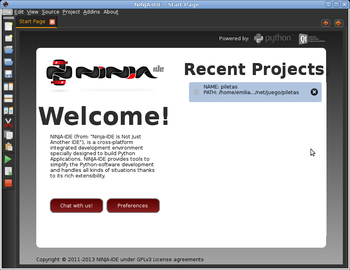
\includegraphics{files/img/u1/ninja-ide.png}
\end{figure}

Un IDE es un entorno que nos facilita las tareas a la hora de programar.
Consiste en la integración de un editor de texto, con características de
resaltado de sintaxis autocompletado -entre otras-, y el intérprete de
Python. Existen cientos de entornos muy buenos, como por ejemplo
\href{https://github.com/spyder-ide/spyder}{Spyder}\footnote{https://github.com/spyder-ide/spyder},
\href{https://www.jetbrains.com/pycharm}{PyCharm}\footnote{https://www.jetbrains.com/pycharm} o
\href{http://ninja-ide.org}{Ninja-IDE}\footnote{http://ninja-ide.org}. Para el presente curso, nos
basaremos en Ninja-IDE, software libre que ha sido desarrollado por la
comunidad de Python Argentina, \href{http://python.org.ar}{PyAr}\footnote{http://python.org.ar}.

Una lista bastante completa sobre las IDEs disponibles pueden
encontrarse en la \href{https://wiki.python.org/moin/IntegratedDevelopmentEnvironments}{wiki oficial de
Python}\footnote{https://wiki.python.org/moin/IntegratedDevelopmentEnvironments}


\section{Algoritmos computacionales}
\label{Unidad01:algoritmos-computacionales}
En forma simplificada, un programa o software es un conjunto de
instrucciones que la computadora puede ejecutar. Este procedimiento
formado por un conjunto de instrucciones es lo que denominamos algoritmo
computacional. Una analogía a un algoritmo computacional es una receta
de cocina, por ejemplo:

\begin{Verbatim}[commandchars=\\\{\}]
Prender el fuego
Salar la carne
Controlar cada 5 minutos hasta que haya brasas
Poner la carne a la parrilla
Cocinar hasta que esté la carne, controlar cada 5 minutos
Dar vuelta la carne
Cocinar hasta que esté la carne, controlar cada 5 minutos
Si falta sal al probar, salar
\end{Verbatim}

En esta receta se ven una serie de instrucciones que deben ser seguidas
en un determinado orden, en algunos casos contamos con ingredientes,
intrucciones, decisiones y acciones que se repiten. No muy distinto a un
programa de computación, comencemos con algunos \emph{ingredientes} simples
de Python y veamos lo que podemos hacer con ellos.


\subsection{El primer programa ``Adiós mundo!''}
\label{Unidad01:el-primer-programa-adios-mundo}
El acercamiento inicial a un lenguaje de programación suele ser con el
archiconocido programa ``Hola mundo''. Consiste simmplemente en un
programa que muestra en pantalla ese mensaje.

Renunciando a cualquier pretensión de originalidad comenzaremos del
mismo modo, pero despidiéndonos. Para esto utilizaremos la instrucción
\emph{print()} pasando el mensaje de despedida entre comillas, a continuación
la instrucción.

\begin{Verbatim}[commandchars=\\\{\}]
\PYG{k}{print}\PYG{p}{(}\PYG{l+s}{\PYGZdq{}}\PYG{l+s}{Adios mundo cruel!}\PYG{l+s}{\PYGZdq{}}\PYG{p}{)}
\end{Verbatim}

Podemos probar la intrucción directamente desde el intérprete, creando
con un editor de texto plano un archivo guardado como \code{chau.py} y
luego ejecutándolo desde la terminal haciendo \code{python3 chau.py}, o
bien utilizando un IDE y haciendo todo desde ahí mismo.

Ahora bien, es muchísimo más lo que podemos hacer programando además de
saludar cordialmente. Veamos los elementos de un programa que nos
permitirán realizar tareas más complejas y entretenidas.


\section{Elementos de un programa}
\label{Unidad01:elementos-de-un-programa}
A continuación veremos los ingredientes fundamentales de un lenguaje de
programación como Python, para llevar a cabo los ejemplos utilizaremos
el intérprete interactivo mejorado ipython.


\subsection{Números y expresiones}
\label{Unidad01:numeros-y-expresiones}
Frecuentemente requerimos resolver cálculos matemáticos, las operaciones
aritméticas básicas son:
\begin{itemize}
\item {} 
adición: +

\item {} 
sustracción: -

\item {} 
multiplicación: *

\item {} 
división: /

\item {} 
módulo: \%

\item {} 
potencia: **

\item {} 
división entera: //

\end{itemize}

Las operaciones se pueden agrupar con parentesis y tienen precedencia
estándar. Veamos unos ejemplos.

\begin{Verbatim}[commandchars=\\\{\}]
In [9]: 1/3
Out[9]: 0.3333333333333333

In [10]: 1//3
Out[10]: 0

In [11]: 10\PYGZpc{}3
Out[11]: 1

In [12]: 4\PYGZpc{}2
Out[12]: 0
\end{Verbatim}

El caso de la potencia, también nos sirve para calcular raices. Veamos
una potencia al cubo y luego una raíz cuadrada, equivalente a una
potencia a la 1/2.

\begin{Verbatim}[commandchars=\\\{\}]
In [13]: 5**3
Out[13]: 125

In [14]: 2**(1/2)
Out[14]: 1.4142135623730951
\end{Verbatim}

Los datos numéricos que obtenidos en las operaciones previas se
clasifican en reales y enteros, en python se los clasifica como float e
int respectivamente, además existe el tipo complex, para números
complejos.

Utilizando la función type() podemos identificar el tipo de dato.
Veamos:

\begin{Verbatim}[commandchars=\\\{\}]
In [15]: type(0.333)
Out[15]: float

In [16]: type(4)
Out[16]: int
\end{Verbatim}


\subsection{Cadenas de carateres}
\label{Unidad01:cadenas-de-carateres}
Además de números, es posible manipular texto. Las cadenas son
secuencias de caracteres encerradas en comillas simples (`...') o dobles
(''...''), el tipo de datos es denominado \emph{str}. Sin adentrarnos en
detalles, que posteriormente veremos, aquí trataremos lo indispensable
para poder desarrollar los primeros programas. Veamos unos ejemplos:

\begin{Verbatim}[commandchars=\\\{\}]
\PYG{g+gp}{\PYGZgt{}\PYGZgt{}\PYGZgt{} }\PYG{l+s}{\PYGZsq{}}\PYG{l+s}{huevos y pan}\PYG{l+s}{\PYGZsq{}}         \PYG{c}{\PYGZsh{} comillas simples}
\PYG{g+go}{\PYGZsq{}huevos y pan\PYGZsq{}}
\end{Verbatim}

Los operadores algebraicos para la suma y multiplicación tienen efecto
sobre las cadenas:

\begin{Verbatim}[commandchars=\\\{\}]
\PYG{g+gp}{\PYGZgt{}\PYGZgt{}\PYGZgt{} }\PYG{l+s}{\PYGZsq{}}\PYG{l+s}{eco }\PYG{l+s}{\PYGZsq{}}\PYG{o}{*}\PYG{l+m+mi}{4}               \PYG{c}{\PYGZsh{} La multiplicación repite la cadena}
\PYG{g+go}{\PYGZsq{}eco eco eco eco \PYGZsq{}}

\PYG{g+go}{\PYGZgt{}\PYGZgt{}\PYGZgt{}\PYGZsq{}yo y \PYGZsq{}+ \PYGZsq{}mi otro yo\PYGZsq{}   \PYGZsh{} La suma concatena dos o mas cadenas}
\PYG{g+go}{\PYGZsq{}yo y mi otro yo\PYGZsq{}}
\end{Verbatim}

Es posible utilizar cadenas de más de una línea, anteponiendo \textbf{triples
comillas} simples o dobles al inicio y al final, por ejemplo (fragmento
del poema de Fortunato Ramos \emph{Yo jamás fui un niño}):

\begin{Verbatim}[commandchars=\\\{\}]
\PYG{l+s+sd}{\PYGZsq{}\PYGZsq{}\PYGZsq{}}
\PYG{l+s+sd}{Mi sonrisa es seca y mi rostro es serio,}
\PYG{l+s+sd}{mis espaldas anchas, mis músculos duros}
\PYG{l+s+sd}{mis manos partidas por el crudo frío}
\PYG{l+s+sd}{sólo ocho años tengo, pero no soy un niño.}
\PYG{l+s+sd}{\PYGZsq{}\PYGZsq{}\PYGZsq{}}
\end{Verbatim}


\subsection{Variables}
\label{Unidad01:variables}
Las variables son contenedores para almacenar información. Por ejemplo,
para elevar un número al cubo podemos utilizar 3 variables, para la base
(\emph{num1}), para el exponenete (\emph{num2}) y para almacenar el \emph{resultado}:

\begin{Verbatim}[commandchars=\\\{\}]
\PYG{n}{num1} \PYG{o}{=} \PYG{l+m+mi}{5}                   \PYG{c}{\PYGZsh{} num1 toma valor 5.}
\PYG{n}{num2} \PYG{o}{=} \PYG{l+m+mi}{3}                   \PYG{c}{\PYGZsh{} num2 toma 3.}
\PYG{n}{resultado} \PYG{o}{=} \PYG{n}{num1}\PYG{o}{*}\PYG{o}{*}\PYG{n}{num2}     \PYG{c}{\PYGZsh{} resultado toma num1 elevado a num2.}
\PYG{k}{print}\PYG{p}{(}\PYG{l+s}{\PYGZsq{}}\PYG{l+s}{El resultado es}\PYG{l+s}{\PYGZsq{}}\PYG{p}{,} \PYG{n}{resultado}\PYG{p}{)}
\end{Verbatim}

El operador igual (=) sirve para asignar lo que está a su derecha, a la
variable que se encuentra a su izquierda. Implementemos la siguiente
ecuación para dos valores de \emph{x}, 0.1 y 0.2.
\begin{gather}
\begin{split}y = (x-4)^2-3\end{split}\notag
\end{gather}
\begin{Verbatim}[commandchars=\\\{\}]
\PYG{n}{x1} \PYG{o}{=} \PYG{l+m+mf}{0.1}
\PYG{n}{y1} \PYG{o}{=} \PYG{p}{(}\PYG{n}{x1}\PYG{o}{\PYGZhy{}}\PYG{l+m+mi}{4}\PYG{p}{)}\PYG{o}{*}\PYG{o}{*}\PYG{l+m+mi}{2}\PYG{o}{\PYGZhy{}}\PYG{l+m+mi}{3}

\PYG{n}{x2} \PYG{o}{=} \PYG{l+m+mf}{0.2}
\PYG{n}{y2} \PYG{o}{=} \PYG{p}{(}\PYG{n}{x2}\PYG{o}{\PYGZhy{}}\PYG{l+m+mi}{4}\PYG{p}{)}\PYG{o}{*}\PYG{o}{*}\PYG{l+m+mi}{2}\PYG{o}{\PYGZhy{}}\PYG{l+m+mi}{3}

\PYG{k}{print}\PYG{p}{(}\PYG{n}{x1}\PYG{p}{,}\PYG{n}{y1}\PYG{p}{)}
\PYG{k}{print}\PYG{p}{(}\PYG{n}{x2}\PYG{p}{,}\PYG{n}{y2}\PYG{p}{)}
\end{Verbatim}

Veremos la siguiente salida por pantalla:

\begin{Verbatim}[commandchars=\\\{\}]
0.1 12.209999999999999
0.2 11.44
\end{Verbatim}

Otros ejemplos utilizando variables que contengan \textbf{cadenas de
caracteres}:

\begin{Verbatim}[commandchars=\\\{\}]
\PYG{n}{cadena1} \PYG{o}{=} \PYG{l+s}{\PYGZsq{}}\PYG{l+s}{siento que }\PYG{l+s}{\PYGZsq{}}
\PYG{n}{cadena2} \PYG{o}{=} \PYG{l+s}{\PYGZsq{}}\PYG{l+s}{nací en el viento }\PYG{l+s}{\PYGZsq{}}

\PYG{n}{cadena3} \PYG{o}{=} \PYG{n}{cadena1} \PYG{o}{+} \PYG{n}{cadena2}

\PYG{k}{print}\PYG{p}{(}\PYG{n}{cadena3}\PYG{p}{)}
\end{Verbatim}

Los nombres de las variables (identificador o etiqueta) pueden estar
formados por letras, dígitos y guiones bajos, teniendo en cuenta ciertas
restricciones, no pueden comenzar con un número y ni ser algunas de las
siguientes palabras reservadas:

\begin{Verbatim}[commandchars=\\\{\}]
False      class      finally    is         return
None       continue   for        lambda     try
True       def        from       nonlocal   while
and        del        global     not        with
as         elif       if         or         yield
assert     else       import     pass
break      except     in         raise
\end{Verbatim}

Se debe tener en cuenta que las variables diferencian entre mayúsculas y
minúsculas, de modo que juana, JUANA, JuAnA, JUANa son variables
diferentes. Esta característica suele denominarse como \emph{case-sensitive}.


\subsection{Lectura de datos}
\label{Unidad01:lectura-de-datos}
De los ejemplos que vimos, los valores que almacenan las variables
fueron ingresadas en el mismo código, difícilmente sea útil contar con
los valores cargados en el programa en forma estática. Por esta razón,
generalmente se requiere leer información de diferentes fuentes, puede
ser desde un archivo o bien interactuando con un usuario.

La lectura de datos desde el teclado se realiza utilizando la sentencia
\emph{input()} del siguiente modo:

\begin{Verbatim}[commandchars=\\\{\}]
\PYG{n}{nombre} \PYG{o}{=} \PYG{n+nb}{input}\PYG{p}{(}\PYG{l+s}{\PYGZdq{}}\PYG{l+s}{¿Cómo es su nombre, maestro? }\PYG{l+s}{\PYGZdq{}}\PYG{p}{)}
\PYG{k}{print} \PYG{l+s}{\PYGZdq{}}\PYG{l+s}{Hola, }\PYG{l+s}{\PYGZdq{}} \PYG{o}{+} \PYG{n}{nombre} \PYG{o}{+} \PYG{l+s}{\PYGZdq{}}\PYG{l+s}{!}\PYG{l+s}{\PYGZdq{}}
\end{Verbatim}

El comportamiento es:

\begin{Verbatim}[commandchars=\\\{\}]
¿Cómo es su nombre, maestro?
Juan de los palotes
Hola, Juan de los palotes!
\end{Verbatim}

Es importante tener en cuenta que toda lectura por teclado utilizando la
función \emph{input()} va a almacenar lo ingresado como una variable de tipo
\emph{str}, es decir una cadena de caracteres. Veamos el comportamiento al
sumar dos números:

\begin{Verbatim}[commandchars=\\\{\}]
\PYG{n}{num1} \PYG{o}{=} \PYG{n+nb}{input}\PYG{p}{(}\PYG{l+s}{\PYGZdq{}}\PYG{l+s}{Ingrese un número = }\PYG{l+s}{\PYGZdq{}}\PYG{p}{)}
\PYG{n}{num2} \PYG{o}{=} \PYG{n+nb}{input}\PYG{p}{(}\PYG{l+s}{\PYGZdq{}}\PYG{l+s}{Ingrese otro número = }\PYG{l+s}{\PYGZdq{}}\PYG{p}{)}
\PYG{k}{print}\PYG{p}{(}\PYG{l+s}{\PYGZdq{}}\PYG{l+s}{El resultado es =}\PYG{l+s}{\PYGZdq{}}\PYG{p}{,} \PYG{n}{num1}\PYG{o}{+}\PYG{n}{num2}\PYG{p}{)}
\end{Verbatim}

\begin{Verbatim}[commandchars=\\\{\}]
Ingrese un número = 28
Ingrese otro número = 03
El resultado es = 2803
\end{Verbatim}

Claramente la suma de los valores ingresados no da el resultado
observado. El inconveniente se debe a que ambos valores son tomados como
cadenas de caracteres y la operación de suma entre cadenas de caracteres
produce la concatenación de las mismas. Es necesaria convertir la cadena
de caracteres (str) a un valor numérico, ya sea entero o real (int o
float).

Para convertir datos de diferentes tipo se utilizan las funciones int(),
float() o str(). Modificando el caso anterior:

\begin{Verbatim}[commandchars=\\\{\}]
\PYG{n}{num1} \PYG{o}{=} \PYG{n+nb}{int}\PYG{p}{(}\PYG{n+nb}{input}\PYG{p}{(}\PYG{l+s}{\PYGZdq{}}\PYG{l+s}{Ingrese un número = }\PYG{l+s}{\PYGZdq{}}\PYG{p}{)}\PYG{p}{)}
\PYG{n}{num2} \PYG{o}{=} \PYG{n+nb}{int}\PYG{p}{(}\PYG{n+nb}{input}\PYG{p}{(}\PYG{l+s}{\PYGZdq{}}\PYG{l+s}{Ingrese otro número = }\PYG{l+s}{\PYGZdq{}}\PYG{p}{)}\PYG{p}{)}
\PYG{k}{print}\PYG{p}{(}\PYG{l+s}{\PYGZdq{}}\PYG{l+s}{El resultado es =}\PYG{l+s}{\PYGZdq{}}\PYG{p}{,} \PYG{n}{num1}\PYG{o}{+}\PYG{n}{num2}\PYG{p}{)}
\end{Verbatim}

\begin{Verbatim}[commandchars=\\\{\}]
Ingrese un número = 28
Ingrese otro número = 03
El resultado es = 31
\end{Verbatim}

Veamos un ejemplo para operar directamente el valor leído en una
ecuación matemática con el siguiente código:

\begin{Verbatim}[commandchars=\\\{\}]
\PYG{n}{x} \PYG{o}{=} \PYG{n+nb}{input}\PYG{p}{(}\PYG{l+s}{\PYGZdq{}}\PYG{l+s}{Ingrese x = }\PYG{l+s}{\PYGZdq{}}\PYG{p}{)}
\PYG{n}{y} \PYG{o}{=} \PYG{p}{(}\PYG{n}{x}\PYG{o}{\PYGZhy{}}\PYG{l+m+mi}{4}\PYG{p}{)}\PYG{o}{*}\PYG{o}{*}\PYG{l+m+mi}{2}\PYG{o}{\PYGZhy{}}\PYG{l+m+mi}{3}
\PYG{k}{print}\PYG{p}{(}\PYG{n}{x}\PYG{p}{,}\PYG{n}{y}\PYG{p}{)}
\end{Verbatim}

\begin{Verbatim}[commandchars=\\\{\}]
Ingrese x = 3
\end{Verbatim}

\begin{Verbatim}[commandchars=\\\{\}]
\PYGZhy{}\PYGZhy{}\PYGZhy{}\PYGZhy{}\PYGZhy{}\PYGZhy{}\PYGZhy{}\PYGZhy{}\PYGZhy{}\PYGZhy{}\PYGZhy{}\PYGZhy{}\PYGZhy{}\PYGZhy{}\PYGZhy{}\PYGZhy{}\PYGZhy{}\PYGZhy{}\PYGZhy{}\PYGZhy{}\PYGZhy{}\PYGZhy{}\PYGZhy{}\PYGZhy{}\PYGZhy{}\PYGZhy{}\PYGZhy{}\PYGZhy{}\PYGZhy{}\PYGZhy{}\PYGZhy{}\PYGZhy{}\PYGZhy{}\PYGZhy{}\PYGZhy{}\PYGZhy{}\PYGZhy{}\PYGZhy{}\PYGZhy{}\PYGZhy{}\PYGZhy{}\PYGZhy{}\PYGZhy{}\PYGZhy{}\PYGZhy{}\PYGZhy{}\PYGZhy{}\PYGZhy{}\PYGZhy{}\PYGZhy{}\PYGZhy{}\PYGZhy{}\PYGZhy{}\PYGZhy{}\PYGZhy{}\PYGZhy{}\PYGZhy{}\PYGZhy{}\PYGZhy{}\PYGZhy{}\PYGZhy{}\PYGZhy{}\PYGZhy{}\PYGZhy{}\PYGZhy{}\PYGZhy{}\PYGZhy{}\PYGZhy{}\PYGZhy{}\PYGZhy{}\PYGZhy{}\PYGZhy{}\PYGZhy{}\PYGZhy{}\PYGZhy{}
TypeError                                 Traceback (most recent call last)

\PYGZlt{}ipython\PYGZhy{}input\PYGZhy{}15\PYGZhy{}3baa5c95d16e\PYGZgt{} in \PYGZlt{}module\PYGZgt{}()
      1 x = input(\PYGZdq{}Ingrese x = \PYGZdq{})
\PYGZhy{}\PYGZhy{}\PYGZhy{}\PYGZhy{}\PYGZgt{} 2 y = (x\PYGZhy{}4)**2\PYGZhy{}3
      3 print(x,y)


TypeError: unsupported operand type(s) for \PYGZhy{}: \PYGZsq{}str\PYGZsq{} and \PYGZsq{}int\PYGZsq{}
\end{Verbatim}

A diferencia del ejemplo visto anteriormente, donde la suma de dos
cadenas era una operación perfectamente válida, ahora nos encontramos
con operaciones entre diferentes tipos pero incompatibles. En este caso,
podemos convertir la entrada en un número flotante para opearar con
normalidad:

\begin{Verbatim}[commandchars=\\\{\}]
\PYG{n}{x} \PYG{o}{=} \PYG{n+nb}{float}\PYG{p}{(}\PYG{n+nb}{input}\PYG{p}{(}\PYG{l+s}{\PYGZdq{}}\PYG{l+s}{Ingrese x = }\PYG{l+s}{\PYGZdq{}}\PYG{p}{)}\PYG{p}{)}
\PYG{n}{y} \PYG{o}{=} \PYG{p}{(}\PYG{n}{x}\PYG{o}{\PYGZhy{}}\PYG{l+m+mi}{4}\PYG{p}{)}\PYG{o}{*}\PYG{o}{*}\PYG{l+m+mi}{2}\PYG{o}{\PYGZhy{}}\PYG{l+m+mi}{3}
\PYG{k}{print}\PYG{p}{(}\PYG{n}{x}\PYG{p}{,}\PYG{n}{y}\PYG{p}{)}
\end{Verbatim}

\begin{Verbatim}[commandchars=\\\{\}]
Ingrese x = 3
3.0 \PYGZhy{}2.0
\end{Verbatim}

Es posible combinar distintos tipos de datos haciendo la conversión
correspondiente, en el último ejemplo, tanto \emph{x} como \emph{y} son de tipo
\emph{float} y es posible concatenarlos a una cadena de caracteres haciendo
la conversión correspondiente, utilizando la función \emph{str()}:

\begin{Verbatim}[commandchars=\\\{\}]
\PYG{n}{mensaje} \PYG{o}{=} \PYG{l+s}{\PYGZsq{}}\PYG{l+s}{y vale }\PYG{l+s}{\PYGZsq{}} \PYG{o}{+} \PYG{n+nb}{str}\PYG{p}{(}\PYG{n}{y}\PYG{p}{)} \PYG{o}{+} \PYG{l+s}{\PYGZsq{}}\PYG{l+s}{ para un valor de x = }\PYG{l+s}{\PYGZsq{}}\PYG{o}{+} \PYG{n+nb}{str}\PYG{p}{(}\PYG{n}{x}\PYG{p}{)}
\end{Verbatim}


\subsection{Escritura de datos}
\label{Unidad01:escritura-de-datos}
Hemos hecho uso de la función \emph{print()} en su mínima expresión. Iremos
viendo diferentes usos a partir de las siguientes variables:

\begin{Verbatim}[commandchars=\\\{\}]
\PYG{c}{\PYGZsh{} Variables a imprimir}
\PYG{n}{cad} \PYG{o}{=} \PYG{l+s}{\PYGZsq{}}\PYG{l+s}{Pi es}\PYG{l+s}{\PYGZsq{}}
\PYG{n}{pi} \PYG{o}{=} \PYG{l+m+mf}{3.1415}
\PYG{n}{mil} \PYG{o}{=} \PYG{l+m+mi}{1000}
\PYG{n}{uno} \PYG{o}{=} \PYG{l+m+mi}{1}
\end{Verbatim}

\textbf{Como argumentos}

La forma más simple es separar los argumentos a ser impresos mediante
comas.

\begin{Verbatim}[commandchars=\\\{\}]
\PYG{k}{print}\PYG{p}{(}\PYG{n}{cad}\PYG{p}{,}\PYG{n}{pi}\PYG{p}{,}\PYG{l+s}{\PYGZsq{}}\PYG{l+s}{aproximadamente}\PYG{l+s}{\PYGZsq{}}\PYG{p}{)}
\end{Verbatim}

\begin{Verbatim}[commandchars=\\\{\}]
Pi es 3.1415 aproximadamente
\end{Verbatim}

Por defecto, la separación que se obtiene entre cada argumento es un
espacio en blanco, sin embargo, se puede cambiar este comportamiento
agregando como argumento \textbf{*sep=' `*} y entre las comillas incluir el
separador deseado, por ejemplo:

\begin{Verbatim}[commandchars=\\\{\}]
print(cad,pi,\PYGZsq{}aproximadamente\PYGZsq{}, sep=\PYGZsq{};\PYGZsq{})
print(cad,pi,\PYGZsq{}aproximadamente\PYGZsq{}, sep=\PYGZsq{},\PYGZsq{})
print(cad,pi,\PYGZsq{}aproximadamente\PYGZsq{}, sep=\PYGZsq{}:\PYGZhy{})\PYGZsq{})
\end{Verbatim}

\begin{Verbatim}[commandchars=\\\{\}]
Pi es;3.1415;aproximadamente
Pi es,3.1415,aproximadamente
Pi es:\PYGZhy{})3.1415:\PYGZhy{})aproximadamente
\end{Verbatim}

Como vemos, en cada ejecución la impresión se realiza en diferentes
renglones, este es el comportamiento por defecto, que puede ser
modificando agregando el parámetro \textbf{*end='' ``*}. Reflejemos esto con un
ejemplo:

\begin{Verbatim}[commandchars=\\\{\}]
print(1, end=\PYGZdq{} \PYGZdq{})
print(2, end=\PYGZdq{} \PYGZdq{})
print(3)
print(4)
\end{Verbatim}

\begin{Verbatim}[commandchars=\\\{\}]
1 2 3
4
\end{Verbatim}

\textbf{Usando comodines}

Los comodines consisten en una marca especial en la cadena a imprimir
que es reemplazada por la variable y el formato que se le indique.
Existen tres tipos de comodines, para números enteros, reales
(flotantes) y para cadenas de caracteres:
\begin{itemize}
\item {} 
Comodín para reales: \%f

\item {} 
Comodín para enteros: \%d

\item {} 
Comodín para cadenas: \%s

\end{itemize}

Se utiliza del siguiente modo:

\begin{Verbatim}[commandchars=\\\{\}]
\PYG{k}{print}\PYG{p}{(}\PYG{l+s}{\PYGZsq{}}\PYG{l+s}{Pi es }\PYG{l+s+si}{\PYGZpc{}f}\PYG{l+s}{ aproximadamente}\PYG{l+s}{\PYGZsq{}} \PYG{o}{\PYGZpc{}}\PYG{n}{pi}\PYG{p}{)}
\PYG{k}{print}\PYG{p}{(}\PYG{l+s}{\PYGZsq{}}\PYG{l+s}{El número }\PYG{l+s+si}{\PYGZpc{}d}\PYG{l+s}{ es }\PYG{l+s+si}{\PYGZpc{}s}\PYG{l+s}{ que }\PYG{l+s+si}{\PYGZpc{}d}\PYG{l+s}{\PYGZsq{}} \PYG{o}{\PYGZpc{}}\PYG{p}{(}\PYG{n}{mil}\PYG{p}{,}\PYG{l+s}{\PYGZdq{}}\PYG{l+s}{menor}\PYG{l+s}{\PYGZdq{}}\PYG{p}{,}\PYG{n}{mil}\PYG{o}{\PYGZhy{}}\PYG{l+m+mi}{1}\PYG{p}{)}\PYG{p}{)}
\end{Verbatim}

\begin{Verbatim}[commandchars=\\\{\}]
Pi es 3.141500 aproximadamente
El número 1000 es menor que 999
\end{Verbatim}

Es posible formatear los valores, elegir el ancho del campo, la cantidad
de decimales, entre muchas otras funciones.

\begin{Verbatim}[commandchars=\\\{\}]
\PYG{k}{print}\PYG{p}{(}\PYG{l+s}{\PYGZsq{}}\PYG{l+s+si}{\PYGZpc{}.2f}\PYG{l+s}{ }\PYG{l+s+si}{\PYGZpc{}.4f}\PYG{l+s}{ }\PYG{l+s+si}{\PYGZpc{}.3f}\PYG{l+s}{\PYGZsq{}} \PYG{o}{\PYGZpc{}}\PYG{p}{(}\PYG{n}{pi}\PYG{p}{,}\PYG{n}{pi}\PYG{p}{,}\PYG{n}{pi}\PYG{p}{)}\PYG{p}{)}
\PYG{k}{print}\PYG{p}{(}\PYG{l+s}{\PYGZsq{}}\PYG{l+s+si}{\PYGZpc{}4d}\PYG{l+s}{\PYGZsq{}} \PYG{o}{\PYGZpc{}}\PYG{n}{uno}\PYG{p}{)}
\end{Verbatim}

\begin{Verbatim}[commandchars=\\\{\}]
3.14 3.1415 3.142
   1
\end{Verbatim}

Algunas variantes de lo visto se explica en la siguiente lista:

\begin{Verbatim}[commandchars=\\\{\}]
\PYGZpc{}d : un entero
\PYGZpc{}5d: un entero escrito en un campo de 5 caracteres, alineado a la derecha
\PYGZpc{}\PYGZhy{}5d: un entero escrito en un campo de 5 caracteres, alineado a la izquierda
\PYGZpc{}05d: un entero escrito en un campo de 5 caracteres, completado con ceros desde la izquierda (ej. 00041)
\PYGZpc{}e: flotante escrito en notación científica
\PYGZpc{}E: como \PYGZpc{}e, pero E en mayúscula
\PYGZpc{}11.3e: flotante escrito en notación científica con 3 decimales en un campo de 11 caracteres
\PYGZpc{}.3e: flotante escrito en notación científica con 3 decimales en un campo de ancho mínimo
\PYGZpc{}5.1f: flotante con un decimal en un campo de 5 de caracteres
\PYGZpc{}.3f: flotante con 3 decimales en un campo de mínimo ancho
\PYGZpc{}s: una cadena
\PYGZpc{}\PYGZhy{}20s: una cadena alineada a la izquierda en un campo de 20 caracteres de ancho
\end{Verbatim}


\subsection{Operadores relacionales y lógicos}
\label{Unidad01:operadores-relacionales-y-logicos}

\subsection{Funciones}
\label{Unidad01:funciones}

\subsection{Módulos}
\label{Unidad01:modulos}

\section{Ejercicios}
\label{Unidad01:ejercicios}

\chapter{Estructuras de control}
\label{Unidad02::doc}\label{Unidad02:estructuras-de-control}

\section{Condicionales}
\label{Unidad02:condicionales}

\subsection{if}
\label{Unidad02:if}

\subsection{else}
\label{Unidad02:else}

\subsection{Estructuras anidadas}
\label{Unidad02:estructuras-anidadas}

\subsection{elif}
\label{Unidad02:elif}

\section{Repeticiones}
\label{Unidad02:repeticiones}

\subsection{while}
\label{Unidad02:while}

\section{Ejercicios}
\label{Unidad02:ejercicios}
\begin{Verbatim}[commandchars=\\\{\}]
\PYG{k}{for} \PYG{n}{i} \PYG{o+ow}{in} \PYG{n+nb}{range}\PYG{p}{(}\PYG{l+m+mi}{1}\PYG{p}{,}\PYG{l+m+mi}{10}\PYG{p}{)}\PYG{p}{:}
    \PYG{k}{if} \PYG{n}{i}\PYG{o}{\PYGZpc{}}\PYG{l+m+mi}{2}\PYG{o}{==}\PYG{l+m+mi}{0}\PYG{p}{:}
        \PYG{k}{print}\PYG{p}{(}\PYG{n}{i}\PYG{p}{,}\PYG{l+s}{\PYGZdq{}}\PYG{l+s}{es par}\PYG{l+s}{\PYGZdq{}}\PYG{p}{)}
    \PYG{k}{else}\PYG{p}{:}
        \PYG{k}{print}\PYG{p}{(}\PYG{n}{i}\PYG{p}{,} \PYG{l+s}{\PYGZdq{}}\PYG{l+s}{es impar}\PYG{l+s}{\PYGZdq{}}\PYG{p}{)}
\end{Verbatim}

\begin{Verbatim}[commandchars=\\\{\}]
1 es impar
2 es par
3 es impar
4 es par
5 es impar
6 es par
7 es impar
8 es par
9 es impar
\end{Verbatim}


\chapter{Más estructuras de datos y control}
\label{Unidad03:mas-estructuras-de-datos-y-control}\label{Unidad03::doc}

\section{Listas}
\label{Unidad03:listas}

\section{for}
\label{Unidad03:for}

\section{Manipulando textos con strings}
\label{Unidad03:manipulando-textos-con-strings}

\chapter{Funciones, archivos, diccionarios}
\label{Unidad04::doc}\label{Unidad04:funciones-archivos-diccionarios}

\section{Definiendo funciones}
\label{Unidad04:definiendo-funciones}

\subsection{Variables globales y locales}
\label{Unidad04:variables-globales-y-locales}

\subsubsection{Agrupando el código en módulos}
\label{Unidad04:agrupando-el-codigo-en-modulos}

\section{Números aleatorios}
\label{Unidad04:numeros-aleatorios}

\section{Lectura y escritura de archivos}
\label{Unidad04:lectura-y-escritura-de-archivos}

\section{Diccionarios}
\label{Unidad04:diccionarios}

\chapter{Clases y objetos}
\label{Unidad05::doc}\label{Unidad05:clases-y-objetos}

\chapter{This is a Title}
\label{example::doc}\label{example:this-is-a-title}
That has a paragraph about a main subject and is set when the `='
is at least the same length of the title itself.


\section{Subject Subtitle}
\label{example:subject-subtitle}
Subtitles are set with `-` and are required to have the same length
of the subtitle itself, just like titles.

Lists can be unnumbered like:
\begin{itemize}
\item {} 
Item Foo

\item {} 
Item Bar

\end{itemize}

Or automatically numbered:
\begin{enumerate}
\item {} 
Item 1

\item {} 
Item 2

\end{enumerate}


\section{Inline Markup}
\label{example:inline-markup}
Words can have \emph{emphasis in italics} or be \textbf{bold} and you can define
code samples with back quotes, like when you talk about a command: \code{sudo}
gives you super user powers!


\chapter{Indices and tables}
\label{index:indices-and-tables}\begin{itemize}
\item {} 
\emph{genindex}

\item {} 
\emph{modindex}

\item {} 
\emph{search}

\end{itemize}



\renewcommand{\indexname}{Índice}
\printindex
\end{document}
